\documentclass{article}
\usepackage[utf8]{inputenc}
\usepackage{pdfpages}
\usepackage{amsmath}
\usepackage{bm}
\usepackage{hyperref}
\usepackage{enumitem}
\usepackage{graphicx}
\usepackage[margin=1in]{geometry}
\usepackage{float}
\usepackage{chngcntr}
\counterwithin{figure}{section}
\graphicspath{ {images/} }
\title{RBE/CS549 Project: Boat Tracking/Detection}
\author{Jordan Burklund \and James Kuszmaul}
\begin{document}
\maketitle

\tableofcontents

\section{Task}

We are currently working on a robotic sailboat for the
International Robotic Sailing Competition (\url{http://sailbot.org}).

In navigating a sailboat, we would like to be able to
detect and maneuver around various objects
that are floating on the surface of the water. As such,
it is desirable to be able to (a) identify and (b)
predict the motion of objects on the water. Computer
Vision is a potentially convenient way to do this.
We are not specifically aware of any particularly
thorough published work on this particular application
(while we have used vision in the past, it has been
extremely simple detection of bright-colored buoys
on the water).

The goal of this project shall be to use some existing
video to try and detect and track objects in video,
and to understand how well we can develop such a
detector without having a labelled dataset. We will,
for the time being, not worry about being able to run
the algorithm in real time onboard the boat (although
practical considerations mean it must be able to
perform fast enough for us to evaluate it).

\section{Data}

We have approximately 240GB of HD video from a GoPro
mounted on the prow of a large motorboat. While we
do not have the processing power to fully take advantage
of every frame of data, we pulled reasonable samples
of data to work with.  Specifically, we generated a test dataset of reduced sized that includes the following important characteristics:

\begin{itemize}
\item With/without land (to see different horizon conditions).
\item Varying amounts of other objects/traffic.
\item Areas with significant camera movement in either pitch or roll (may extend to both pitch and roll depending on progress).
\item Different water conditions (starting with flat, calm water, and progressing to more chaotic water conditions as time allows)
\item Objects both near/far away (including near the horizon)
\item Frames that include water droplets on the lens
\end{itemize}

The boat that the data is collected on is relatively stable
and the GoPro is mounted in the same spot for the length
of the video. As such, we should be able to safely ignore
the rotational pose of the boat (when we apply these
algorithms to our final boat, we will have to account for
the much more noticeable movement of that boat).
\begin{figure}[H]
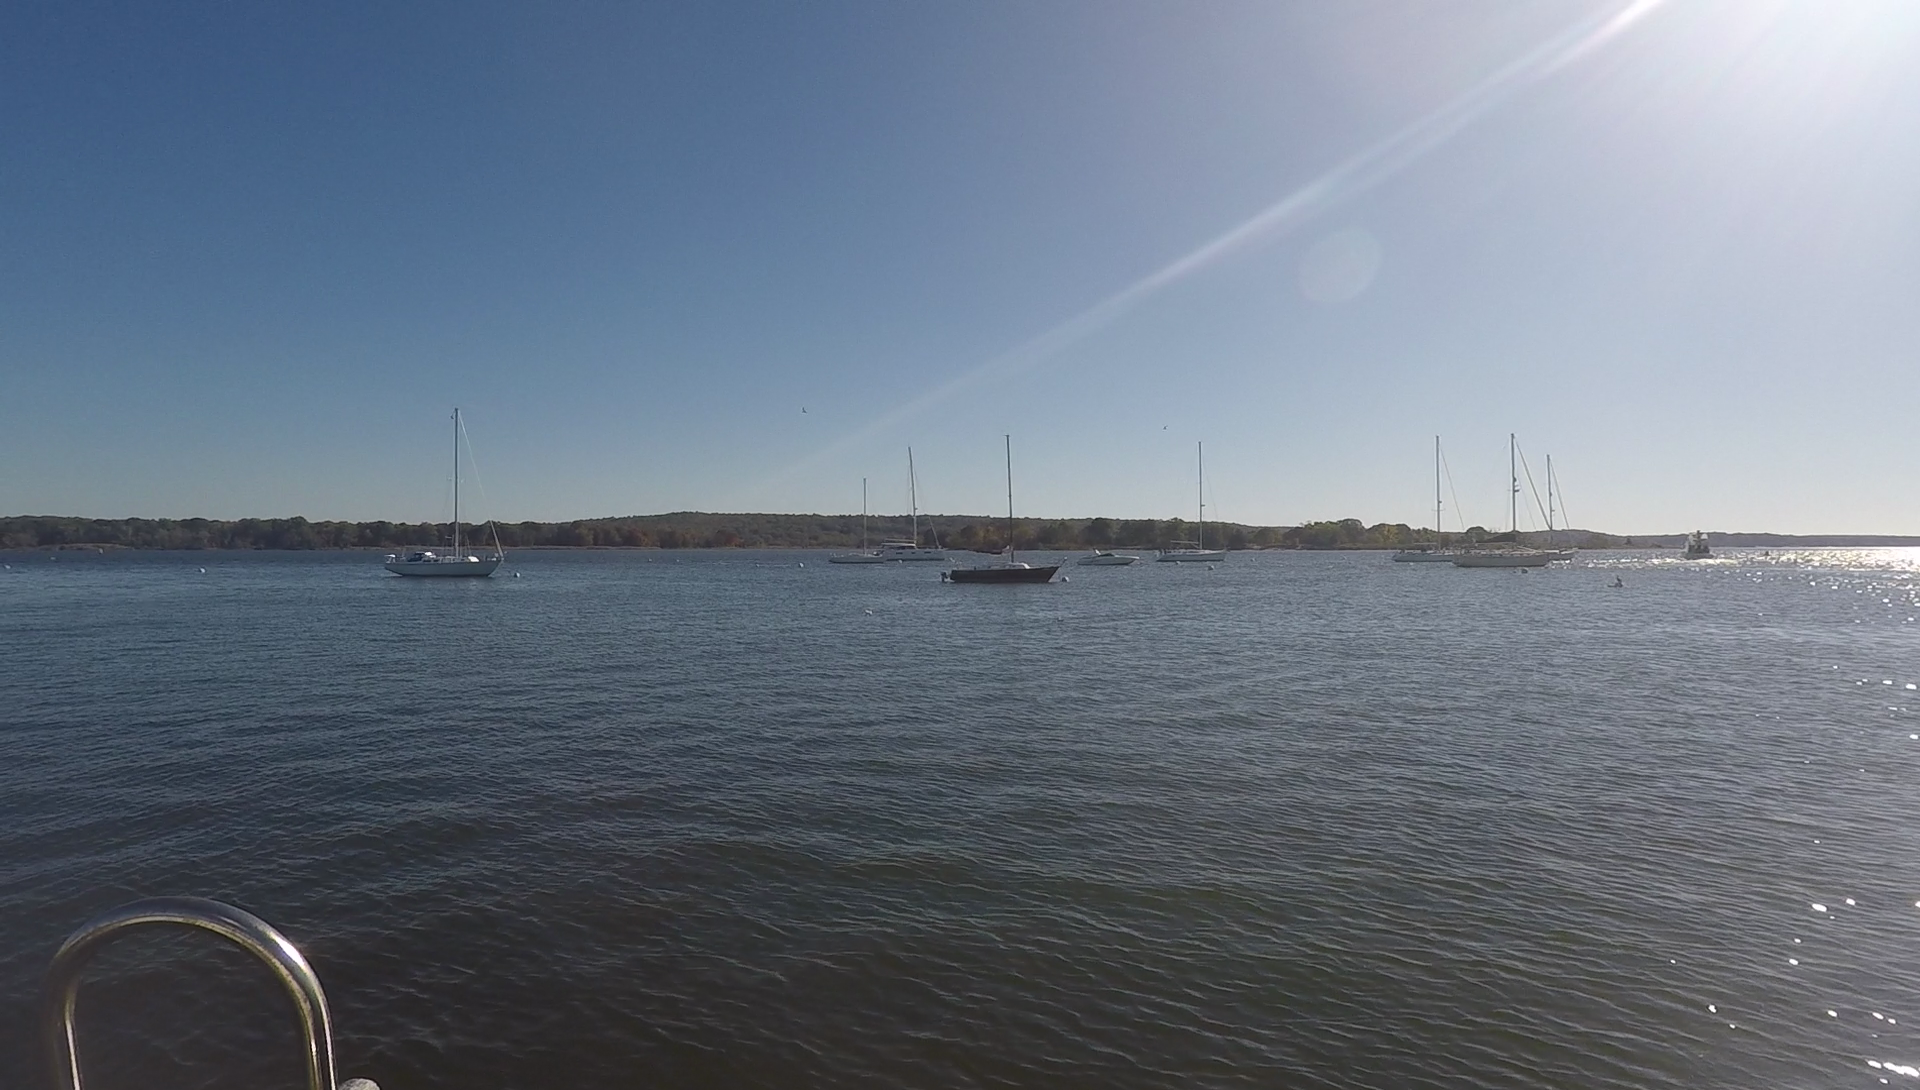
\includegraphics[width=12cm]{sample2}
\centering
\caption{Sample image 1}
\end{figure}


\section{General Approach}

Overall, the object pipeline is as follows:
\begin{figure}[H]
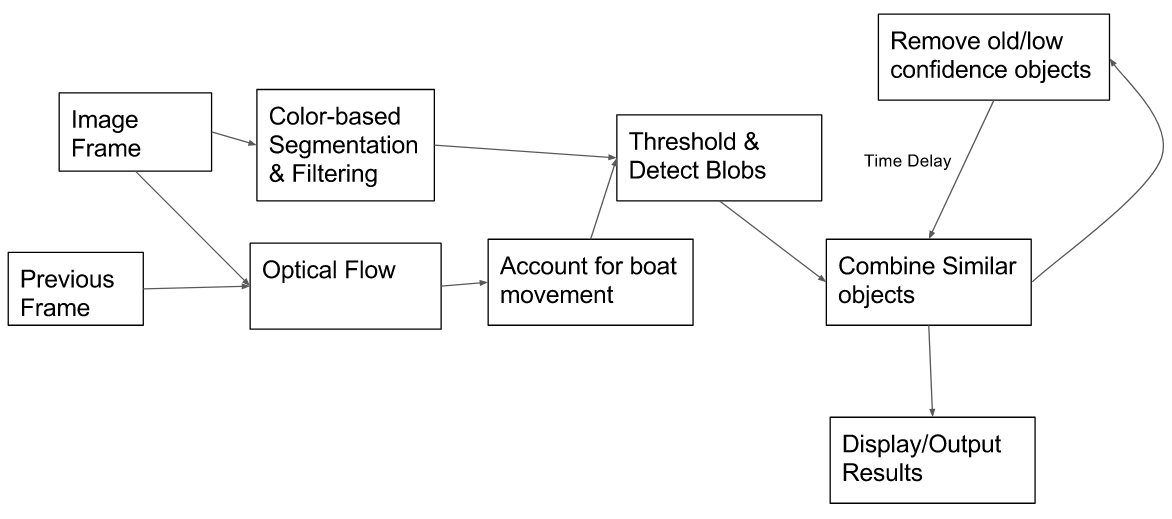
\includegraphics[width=16cm]{algorithm_flowchart}
\centering
\caption{High-Level Image Processing Pipeline}
\end{figure}


\begin{enumerate}
\item We read a frame of video and convert it to HSV space
\item Perform a slew of static transforms to try and determine,
      based on the content of a single frame, which areas are and
      are not water/sky/land/objects
\item Use optical flow information from a given pair of frames to
      locate the moving objects in a frame
\item Combine the above to determine a set of viable blobs
\item Associate the blobs with each other and with preexisting objects,
      creating new objects for blobs that can't be associated with any
      preexisting objects
\item Update objects in preparation for the next frame, updating
      positions using velocities, reducing and increasing confidence
      scores as appropriate, deleting objects with sufficiently low
      scores
\end{enumerate}

\section{Pixel Level Water Segmentation}
In the first part of the pipeline, we look at individual images and attempt to
provide a pixel level detection of potential objects to track.  This step of the
pipeline provides a confidence value for each pixel in the frame for confidence
that the pixels is an object to track.
The image is converted to HSV color space from the original RGB color space since
this gives us better segmentation results. The HSV space has better color
properties for segmentation since the water is typical near one particular
color, but can have variations in brightness.  This also allows the segmentation
to easily segment non-water pixels by the hue value, since the water tends to be
near the blue and green hue values in our test images.

\subsection{Na\"ive K-Means Classifier}
We initially started with a basic two-class k-means classifier in order to
observe how well it would perform.  The classifier was trained on the first
image in the video sequence, and the L2 distance to the two cluster centers was
used to classify each pixel in subsequent frames.  Surprisingly enough, the
2-class k-means classifier worked relatively robustly on the videos that we
provided the algorithm, as show in figure \ref{fig:kmeans}.  The water pixels
are mostly labeled correctly, and pixels that are not water are mostly labeled correctly with a little bit of misclassification noise.  The boat and it's
wake are clearly labeled as potential obstacles to track, which is what we want.
The land areas are labeled as water pixels, but for our implementation we want
to ignore tracking the land anyways. There is a slight bit of noise in the water
reflections towards the right side of figure \ref{fig:kmeans}, but this na\"ive
method still provides very useful information.

K-means does not always associate the same class identifier with the water and
non-water pixels each time, so we must perform an intermediary step to detect
which class identifier it associates with water pixels.  To do so, we find the
number of pixels in each class in the bottom half of the image, and use the sums
to vote for which class is associated with water pixels. This assumes that the
boat is upright, and that a majority of the pixels in the bottom half of the
image are water, which holds true for all of the cases we observed.  If the water
class ID is not what was expected, the cluster centers are swapped so that the
water class ID is always a known value.

\begin{figure}[H]
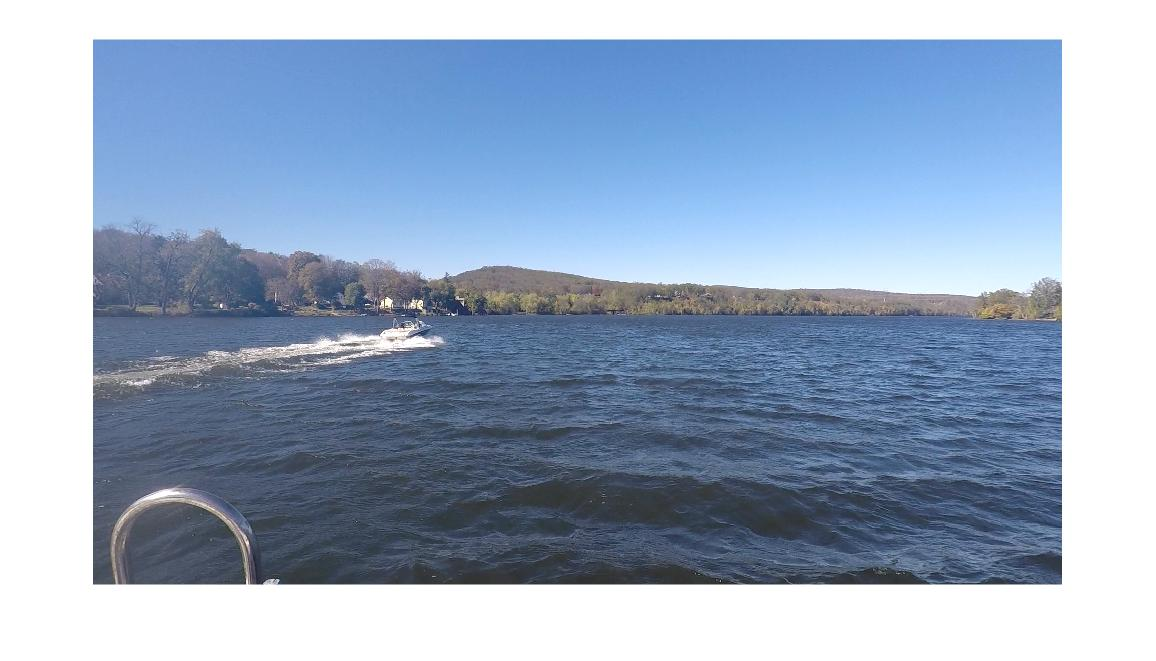
\includegraphics[width=7.8cm]{hsv_kmeans2_orig}
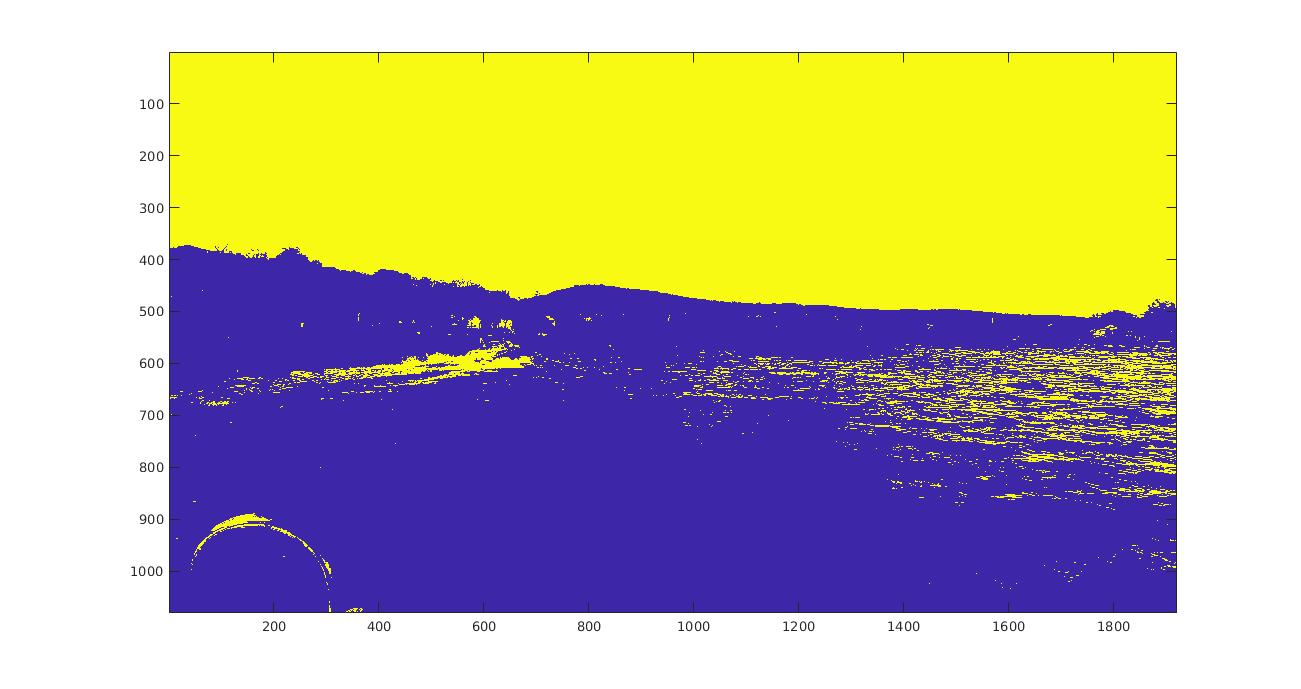
\includegraphics[width=8.5cm]{hsv_kmeans2_result}
\centering
\caption{Na\"ive K-Means Classifier Results}
\label{fig:kmeans}
\end{figure}

\subsection{Wave Reflection Suppression}
Although there is some noise in the classification results, the k-means
classifier does a decent job of selecting pixels that are areas of water. In
order to suppress false detections as seen in the right side of the classifier
results in figure \ref{fig:kmeans}, we look at the distance values between the
pixel's HSV value and the water pixel cluster center to estimate how similar the
pixel is to the water class.  The wave reflections observed in figure
\ref{fig:kmeans} tend to be very close to the cluster center while true obstacle
pixels tend to be further away from the cluster center.  By using this measure
as a confidence value, we can suppress regions that are more likely to be water,
and emphasize regions that are more likely to be objects to track.  Using the
distance metric directly provided decent results, but squaring the distance
metric value provided significantly better suppression of water and emphasis of
potential objects.  The squared value was then used as a direct measure of
confidence that each pixel was a potential object to track.

\subsection{Sky Suppression}
The k-means classifier provides information about which pixels are water and
which pixels are not water, but we would also like the algorithm to only focus
on potential obstacles in the water.  The region of the sky shown in figure
\ref{fig:kmeans} is classified as a non-water pixels, and we would like to
suppress this response to avoid detecting the sky as an obstacle. With only the
wave reflection suppression confidences, most of the sky is suppressed, but
tends to have higher confidences near land as shown in figure
\ref{fig:skysuppress}.  Since the sky pixels are all connected, and define a
very large region, we used the Matlab \texttt{bwareaopen} function that removes binary
pixels in connected areas that are smaller than a particular size.  By looking
only at pixels that are classified as "not water", we can detect the sky region
by filtering for pixel clusters that are larger than 1/4 of the area of the
image, and set the confidence values for those pixels to zero to suppress them.
In some cases, potential objects to track were touching the sky region and the
\texttt{bwareaopen} results tended to remove those object to track.  To fix this, an
erode operation is performed on the non-water class pixels to better separate the sky
and potential objects to track.

\begin{figure}[H]
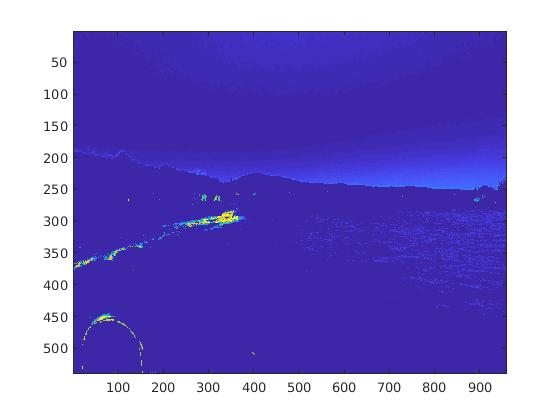
\includegraphics[height=5cm]{hsv_confidence}
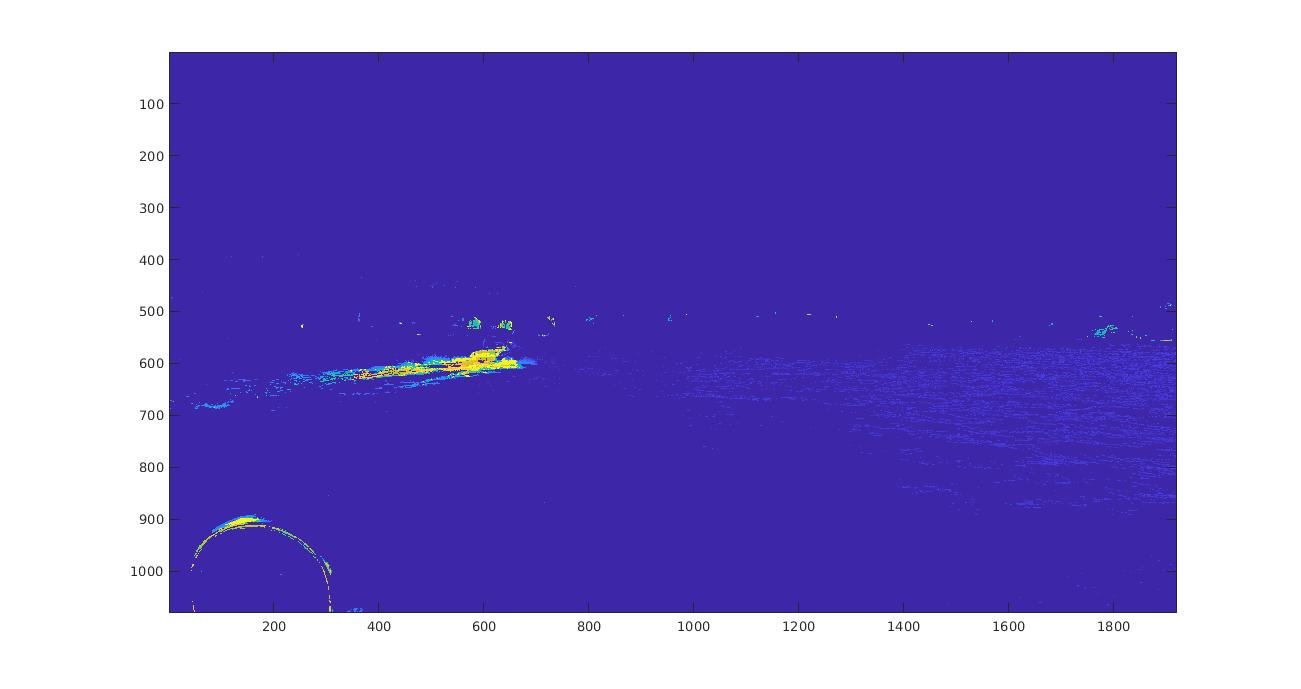
\includegraphics[height=5cm]{hsv_kmeans2_suppressed}
\centering
\caption{Sky Suppression Before and After}
\label{fig:skysuppress}
\end{figure}

\subsection{Confidence Image Results}
When the above confidence values and suppressions described above are combined,
a final confidence value image is produced. Pixels that are more likely to be
objects to track have higher confidence values than pixels that are more likely
to be water areas. Figure \ref{fig:boatconf} shows the detector correctly
detecting a boat in the image.  Figure \ref{fig:towerconf} shows the detector
correctly detecting a tower in the distance.  Figure \ref{fig:buoyconf} shows
the detector identifying a buoy off in the distance.

\begin{figure}[H]
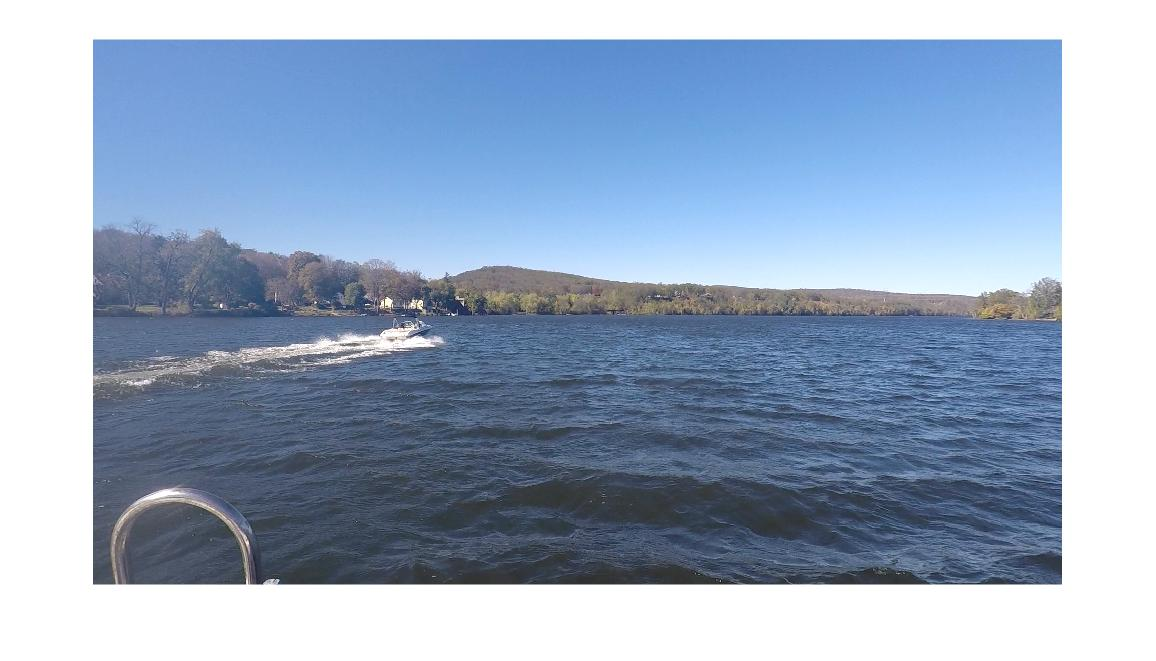
\includegraphics[width=7.8cm]{hsv_kmeans2_orig}
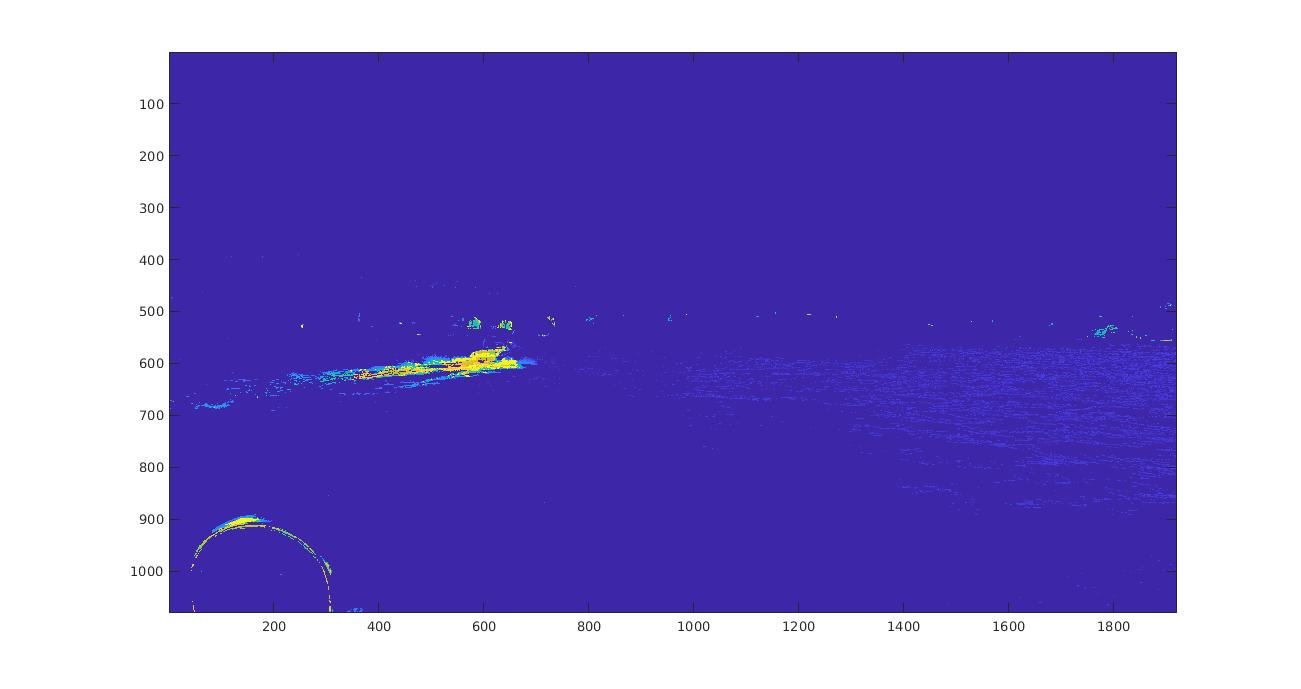
\includegraphics[width=8.5cm]{hsv_kmeans2_suppressed}
\centering
\caption{Boat Confidence Results}
\label{fig:boatconf}
\end{figure}

\begin{figure}[H]
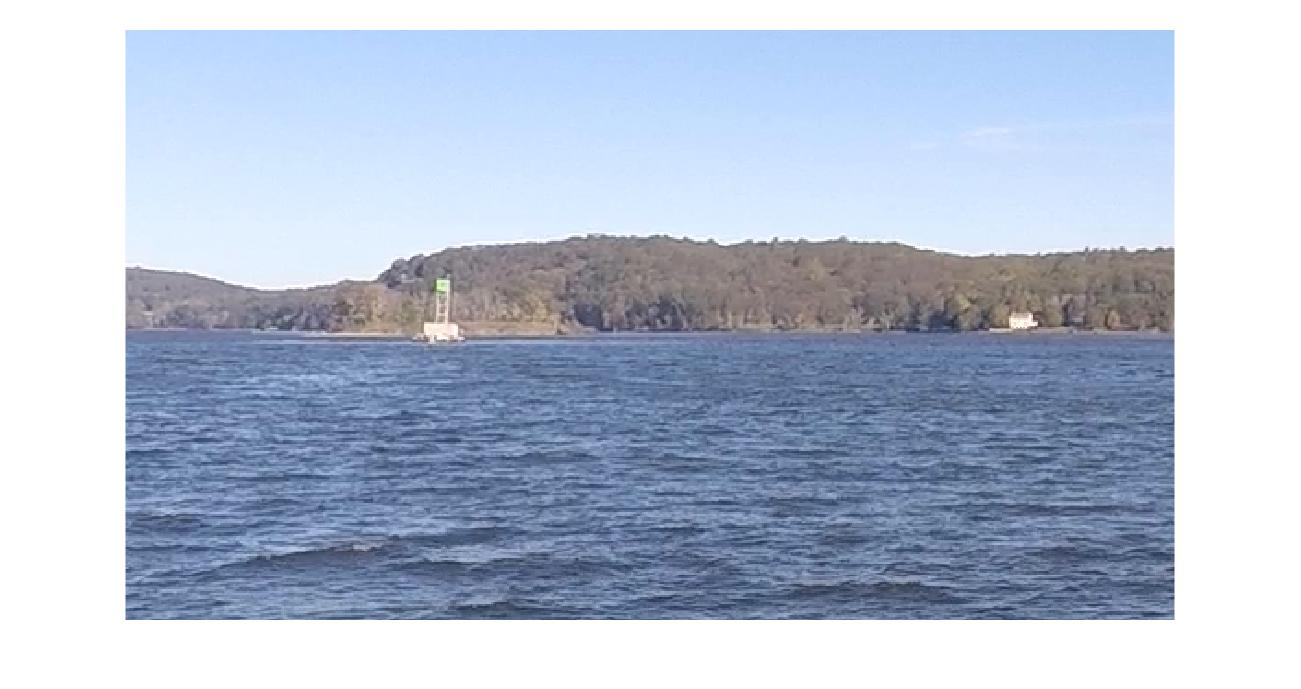
\includegraphics[width=7.9cm]{hsv_kmeans2_tower}
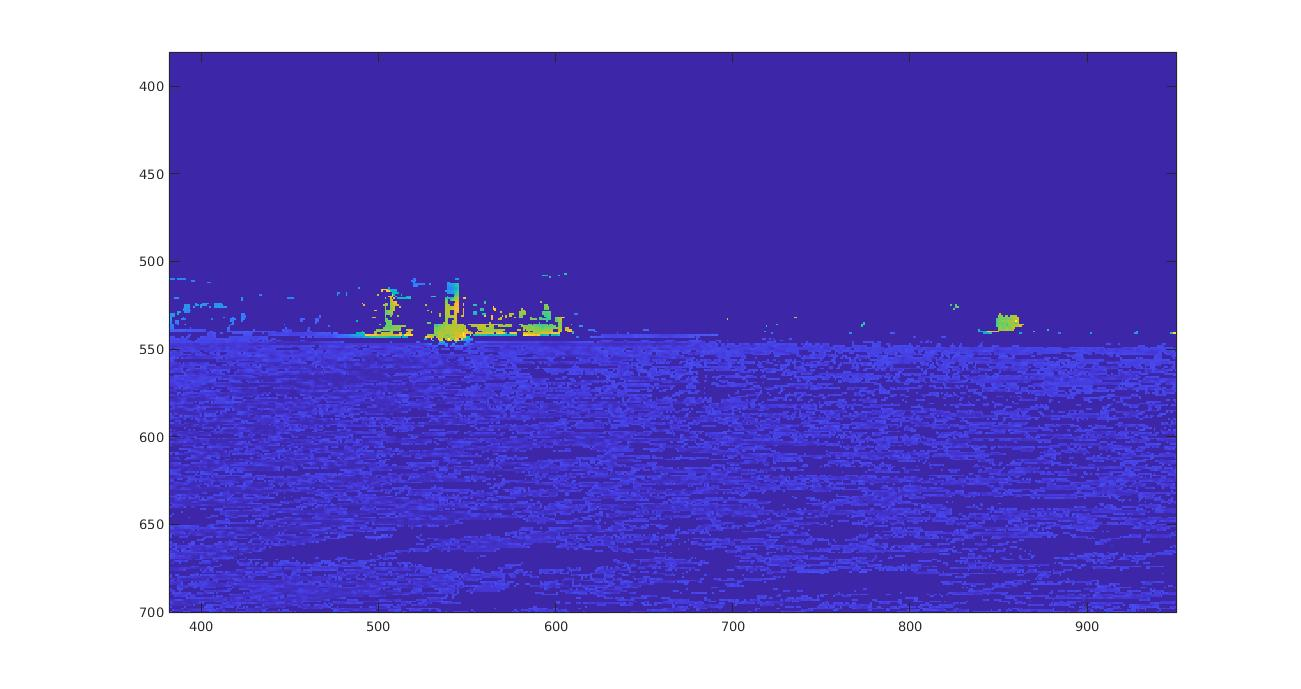
\includegraphics[width=8.3cm]{hsv_kmeans2_tower_result}
\centering
\caption{Tower Confidence Results}
\label{fig:towerconf}
\end{figure}

\begin{figure}[H]
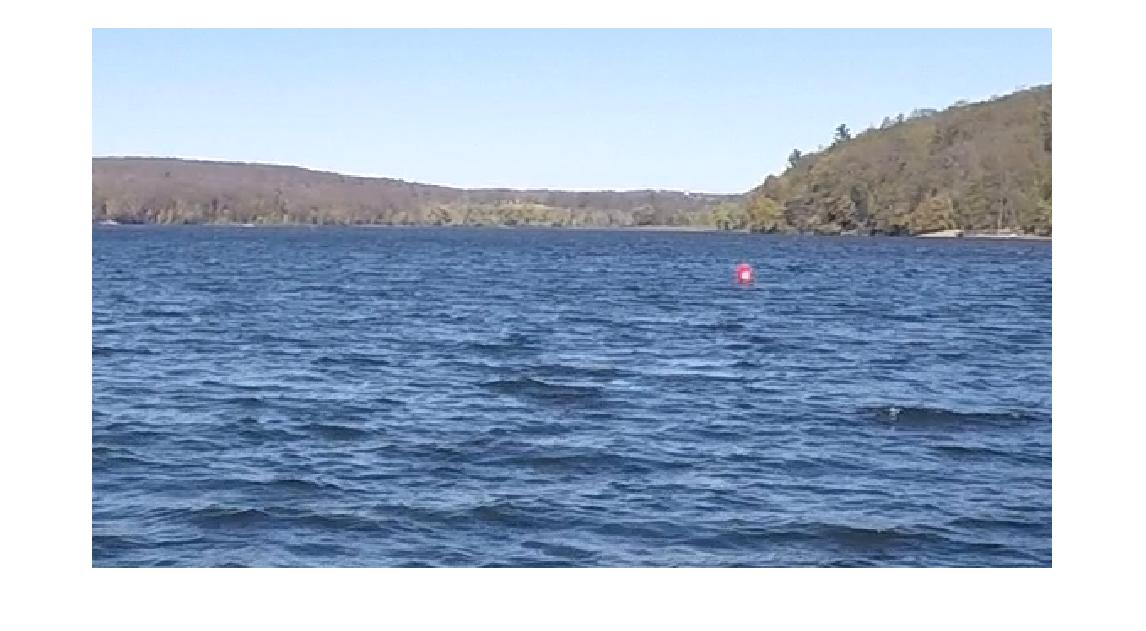
\includegraphics[width=7.8cm]{hsv_kmeans2_buoy}
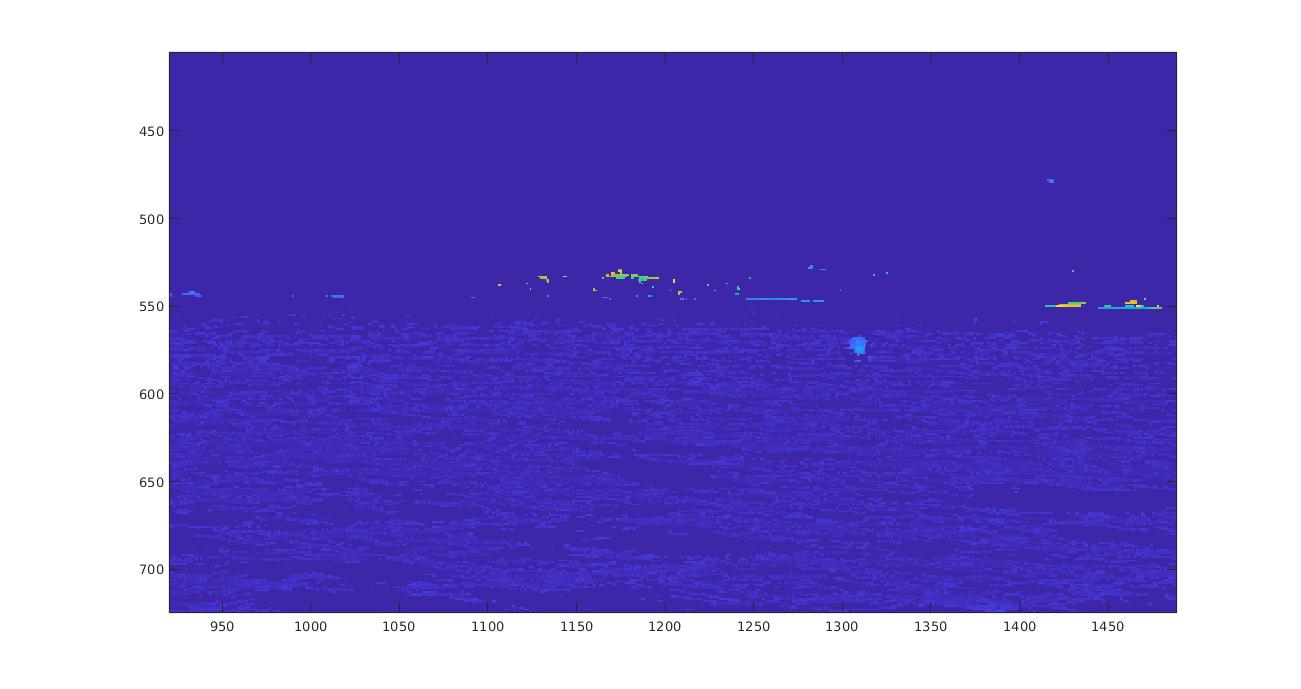
\includegraphics[width=8.5cm]{hsv_kmeans2_buoy_result}
\centering
\caption{Buoy Confidence Results}
\label{fig:buoyconf}
\end{figure}

\section{Optical Flow}

\subsection{Underlying Algorithm}

For the underlying optical flow algorithm, we use Farneback's
\cite{farneback2003} which is accessible in Matlab as
\texttt{opticalFlowFarneback}.

As an overview, the way that this optical flow algorithm works is to
approximate the neighborhood of every pixel as some quadratic function
$f(\mathbf{x}) = \mathbf{x}^T \mathbf{A} \mathbf{x} + \mathbf{b}^T \mathbf{x} + c$
where $\mathbf{x}$ is the location around any given pixel. By estimating these
polynomials about any given pixel between two frames, we can try to estimate how
much the image has moved in the neighborhood of that pixel. Actual
implementations of the algorithm contain some additional filtering/smoothing and
function on multiple levels of an image pyramid to estimate optical flow at
different scales. You can also adjust how much of the neighborhood around a
pixel is used to estimate the polynomial, and various other optimizations.

In practice, we just used the default options to the Matlab method (which uses
a 3-level pyramid scaling image size by a factor of 2, with a 5-pixel
neighborhood size and a Gaussian filter on the output of size 15x15), as these
options tended to produce good results.

\subsection{Expected Flow} \label{expected_flow}

\begin{figure}[H]
\centering
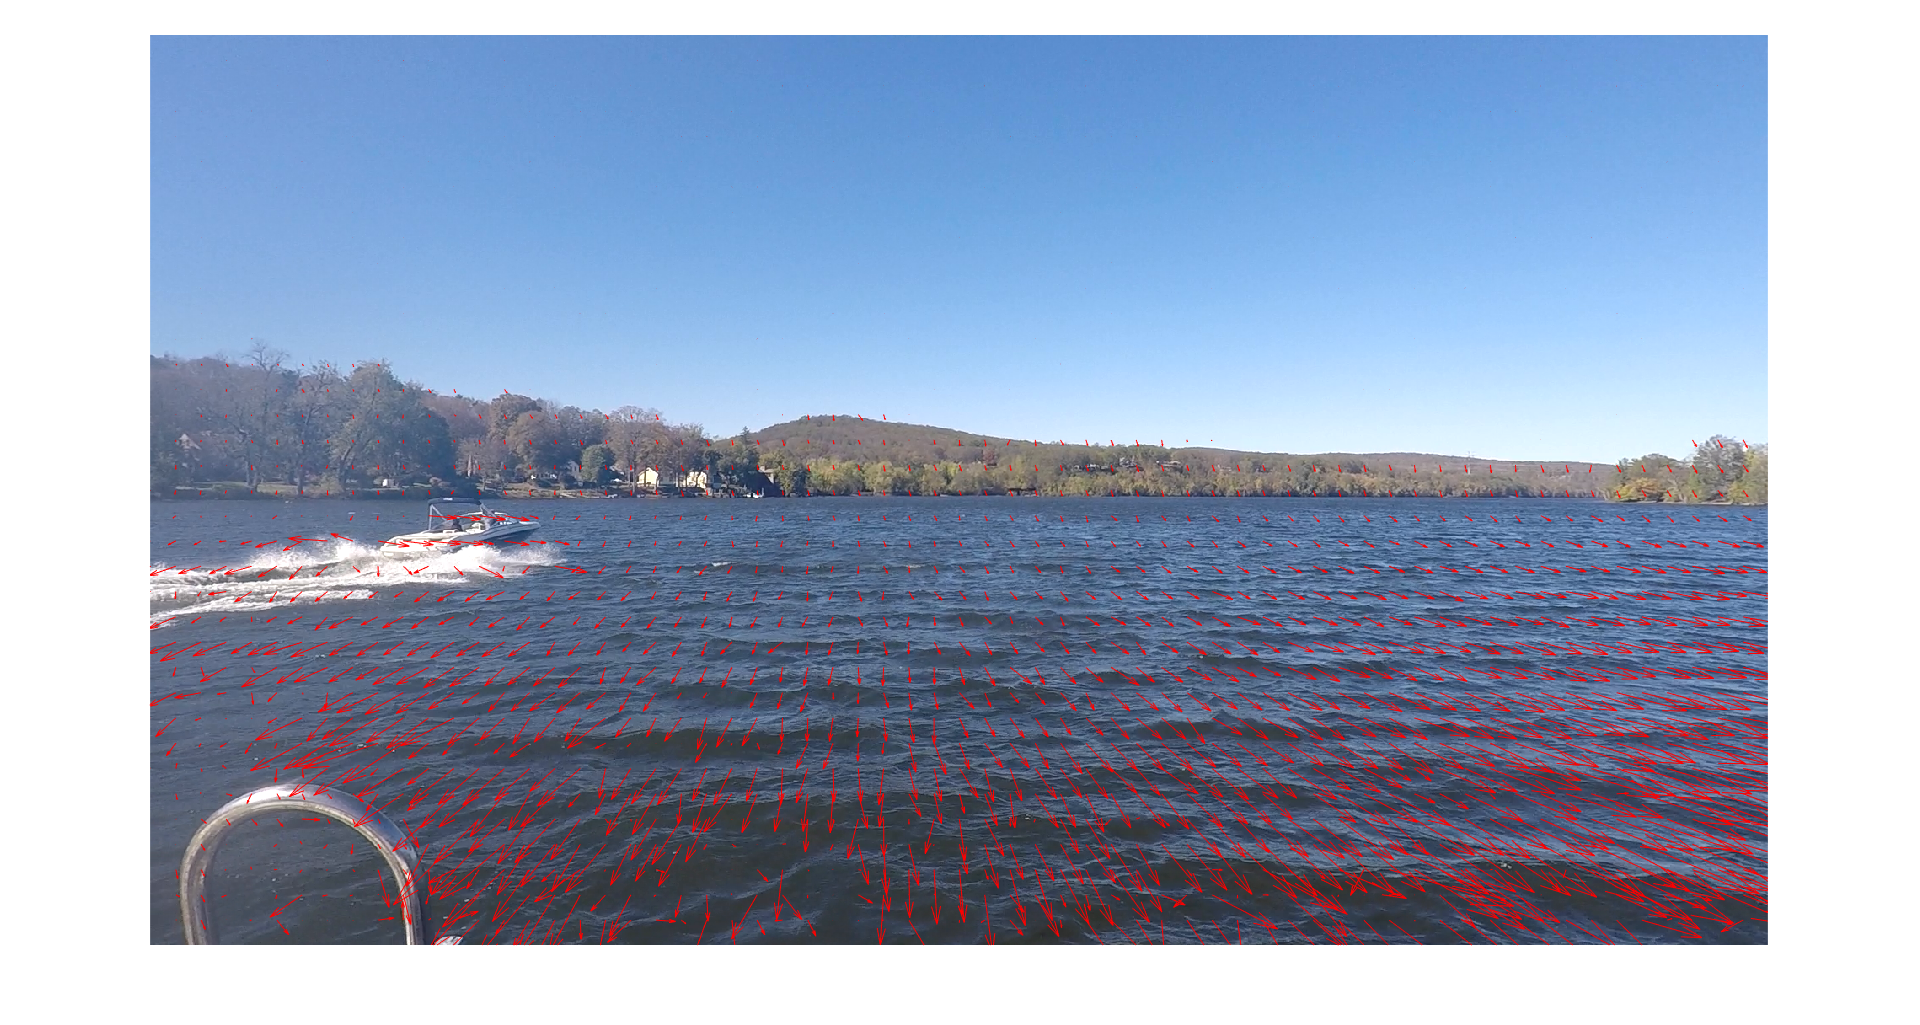
\includegraphics[width=0.7\textwidth]{example_flow.png}
\caption{Optical Flow output (shown only for every few pixels) between two
frames}
\label{fig:example_flow}
\end{figure}

In Figure \ref{fig:example_flow} we show the output of
\texttt{opticalFlowFarneback} on a given pair of frames. The most immediate need
in this image is to try and account for the field of flow produced along the
water. This corresponds to the real movement of the plane of the water relative
to the boat. We can attempt to model this with the following assumptions:
\begin{itemize}
\item That the camera is pointed straight and level
\item There is no substantial roll or yaw angular rates of turn occurring
\item The camera is an ideal pinhole camera with no substantial lens distortions
\item There is no sideways relative velocity between the boat and the water
\end{itemize}

We can define the following variables:

\begin{tabular}{c|c}
Name & Description \\ \hline
$h$ & Height of the camera above the water \\
$v_h$ & The current upwards velocity of the camera \\
$v_b$ & Forwards velocity of the boat relative to the water \\
$x_b, y_b$ & Position coordinates in the boat frame \\
$x_f, y_f$ & X and Y position in the 2-D image frame \\
$\dot{x}_f, \dot{y}_f$ & The expected optical flow (derivatives of $x_f, y_f$)
\\
$K$ & Some constant describing the field of view of the camera \\
\end{tabular}

The boat frame has an origin immediately below the camera on the surface of
the water, is attached to the boat, has an x-axis pointing straight forwards,
a y-axis pointing straight port (left in the camera view) and a z-axis pointing
straight upwards, with the camera at position $(0, 0, h)$ in this frame.

The image frame is scaled so that the center of the image is the origin and
the image is exactly 1 unit tall, with the x-axis being the side-to-side axis
and the y-axis being up-and-down.

Strictly speaking $K = 2\sin\frac\theta2$ if the total vertical field-of-view
of the camera is $\theta$, but we end up estimating it anyways.

These give us:

\begin{align*}
x_f =& \frac{-y_b}{Kx_b} \\
y_f =& \frac{-h}{Kx_b} \\
\dot{x}_f =& \frac{-y_bv_b}{Kx^2_b} \\
\dot{y}_f =& -\frac{1}{Kx_b}(\frac{hv_b}{x_b} + v_h) \\
\end{align*}

And solving for $x_b, y_b$ in terms of $x_f, y_f$ and then substituting in to
give us the expected optical flow at any given image coordinate $x_f, y_f$ we
get:

\begin{align}
\dot{x}_f =& \frac{-v_bKx_fy_f}{h} \\
\dot{y}_f =& \frac{v_hy_f - Kv_by_f^2}{h}
\end{align}

If we ignore the actual values of the constants and just turn them into
something to be estimated, while also adding in a parameter where we
assume that $y_f$ may not be perfectly centered, we can turn this into a
linear parameter estimation problem as:

\begin{align}
\dot{x}_f =& ax_fy_f + bx_f \\
\dot{y}_f =& cy_f^2 + dy_f + e
\end{align}

To actually perform the least-squares fitting we use \texttt{fitlm} in
Matlab. Normally, this just uses a normal least-squares estimation
(similar to doing \texttt{A \ b}), but adds some additional
options. We tried to make use of these options, including a outlier
rejection algorithm, but the effects were minimal and substantially
increased the processing time required to execute the code.

\begin{figure}
\centering
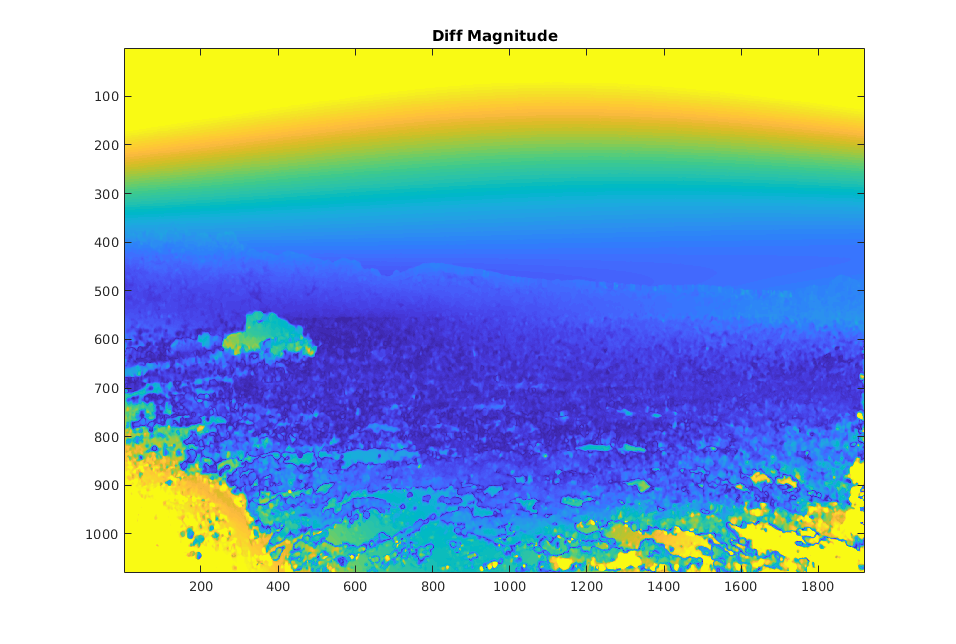
\includegraphics[width=0.6\textwidth]{diff_magnitude}
\caption{Difference between the measured and modelled optical flow.
         Dark blue means perfect match, bright yellow means a poor match.}
\label{fig:diff_magnitude}
\end{figure}

When we compare the expected magnitude of the optical flow to the
actual magnitude of the optical flow in Figure \ref{fig:diff_magnitude}
(this is the same image as Figure \ref{fig:example_flow}),
in which you can see a few features:
\begin{itemize}
\item The boat in the left half of the image shows up as a cyan blob, distinct
      from the water around it.
\item The curved metal in the bottom left affects the optical flow
      algorithm, causing substantial variation from the model.
\item In the bottom right, due to either lens distortion or hard to measure
      waves, the optical flow varies substantially from the model.
\end{itemize}

Due to the poor results in the very bottom of the image and in the
area around the metal bar, we completely ignore and filter out these regions,
as they are relatively unlikely to contain obstacles (or if they did, our
boat would be running them over anyways).

We also note that, in general, objects appearing more distantly in the center of
the image will be hard to identify, as the absolute value of the difference
in magnitude from the modelled magnitude will be low (because we are looking
at optical flow in the image, not real life, so far away objects have
low velocities in the image), and so simple thresholds will not work well.
We experimented with reducing the required threshold in the center of the image,
which did improve tracking.

It is also the case that any stationary, low-lying obstacles (e.g. buoys)
will be indistinguishable from the water and so will not be detected
by this half of the filtering.

\section{Object Creation and Management}

\subsection{Blob Detection and Filtering}

\begin{figure}
\centering
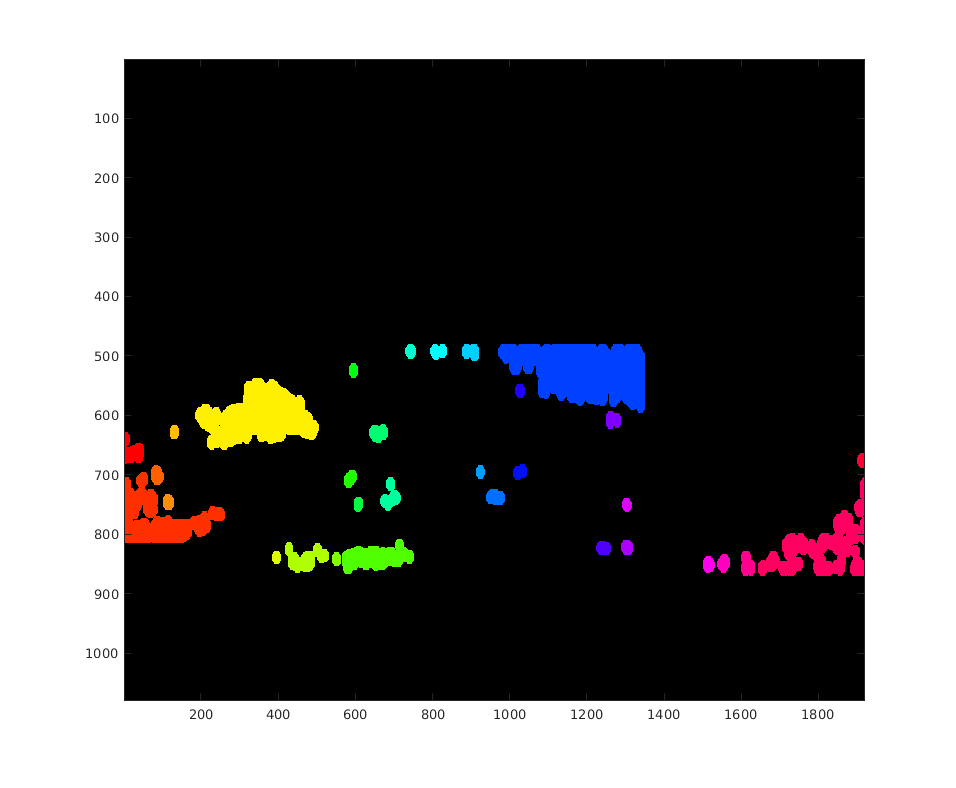
\includegraphics[width=0.5\textwidth]{threshold_bwlabel}
\caption{Result of thresholding after dilation/labelling}
\label{fig:threshold_bwlabel}
\end{figure}

From the results in Figures \ref{fig:boatconf} and
\ref{fig:diff_magnitude}, we have a set of confidence values that can be used to
identify where individual obstacles may be. In order to combine the two, we
simply scale each result by some constant and sum the two to provide a
detection score. Given this score, we then:
\begin{enumerate}
\item Threshold against some constant (tunable) value
\item Do an erode operation using a circular erosion pattern
\item Do a dilate in reverse, using a radius roughly twice that of the erosion,
      so that not only is lost space taken up but nearby segments are connected.
\item Label the connected regions using \texttt{bwlabel} (corresponding with
      Figure \ref{fig:threshold_bwlabel}).
\item For each of these regions, throw out any regions that meet any of the
      following conditions (resulting in Figure \ref{fig:filtered_labels}:
  \begin{itemize}
    \item The object is too ``blue'' (by comparing to some hue-based value,
          in order to try and filter out any water that got detected)
    \item The object is too small (suggesting it may not really exist)
    \item The object is too large (sometimes large (~half the image) connected
          segments will appear that are virtually never real objects)
    \item It is moving too slowly relative to us (relative to the camera,
          the only things that should be that constant are on our
          boat---anything else should at least contain some noise)
  \end{itemize}
\end{enumerate}

\begin{figure}
\centering
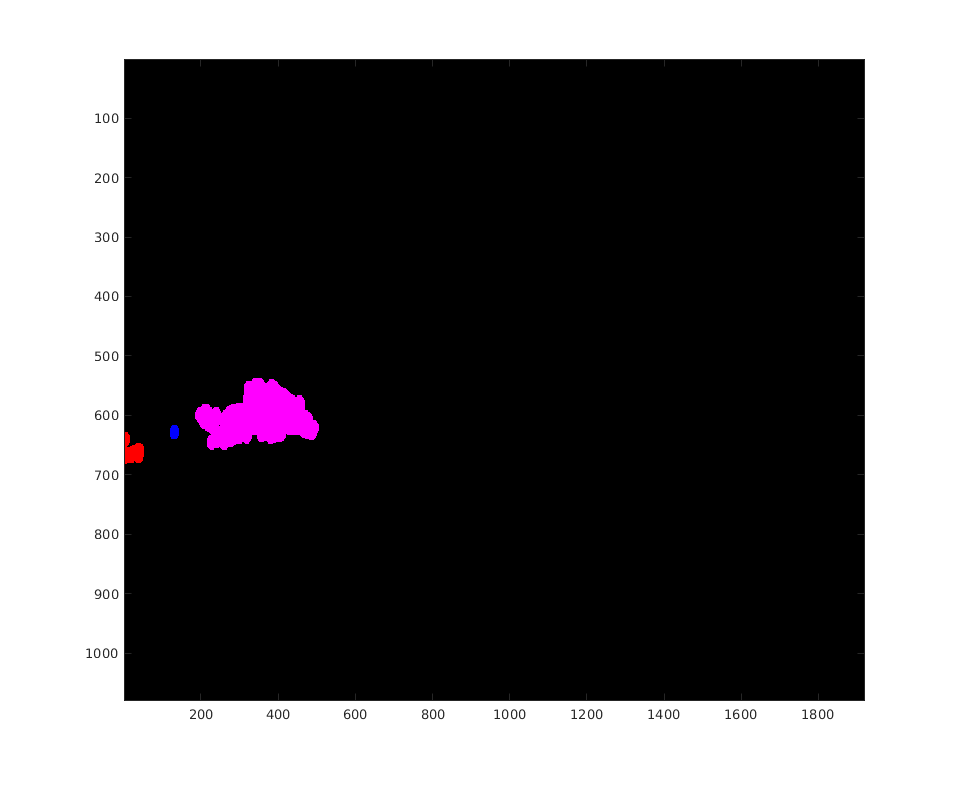
\includegraphics[width=0.5\textwidth]{filtered_labels}
\caption{Result of filtering the blobs in Figure \ref{fig:threshold_bwlabel},
         with the boat and parts of its wake remaining}
\label{fig:filtered_labels}
\end{figure}

Following these steps, we initialize each remaining blob as an object, reducing
it to a bounding box (rather than an exact set of pixels), a median velocity
(from the optical flow), a position (the center of the bounding box), a label
(arbitrarily assigned), and a confidence score (initialized to 0.2, to represent
an object that we are not entirely sure exists yet).

We then go through and, for each object, attempt to both associate it with other
newly created objects (in case any objects were over-segmented) as well as
objects that we've kept track of from the previous frame.

\subsection{Object Matching}

When attempting to match objects, we first update all the old objects so that
their positions have been shifted by their velocities, to better match objects
that are moving between frames. Furthermore, we reduce the bounding box sizes on
old objects to reflect a greater uncertainty; if the object really does exist
over the entire previous bounding box, then that should be reaffirmed by any
blobs detected in the current frame.

We then perform the following steps:

\begin{enumerate}
\item For each pair of new objects, as well as each pairing of one new and one
      old object, we compute a difference score that is the sum of:
  \begin{itemize}
  \item The difference in velocity direction
  \item One minus the quotient in velocity magnitudes (speed), such that the
        larger of the two speeds shall always be in the denominator
  \item The difference in the positions (L2-norm) of the two objects, scaled
        along each axis by the mean width and mean height between the two
        objects (such that if the objects are perfectly aligned in one dimension
        and touching edges in the other, they will be a distance of 1.0 apart).
  \end{itemize}
\item We threshold every difference, leaving a matrix of object ``neighbors''.
\item Iterating over the newly created objects (in arbitrary order), we
      combine that object with it's immediate neighbors, and then remove
      all the objects that were combined from future
      consideration\footnote{Ideally, we might do some sort of search where we
      combine neighbors-of-neighbors and so on, but for simplicities' sake, and
      to avoid situations where we end up combining large numbers of objects
      that all are tenuously connected, we just explore one step out from any
      given object.}.
\item In order to combine each set of objects that we associated, we:
  \begin{itemize}
    \item Create a bounding box that surrounds all of the combined objects
    \item Give the amalgamation the label (and time-of-existence) of the oldest
          object being included, on the assumption that we are interested
          in maintaining tracking going across the longest period of time possible.
    \item Perform a weighted average of the velocities, weighting by object area.
    \item Take the maximum of the confidence scores for the individual objects,
          assign it to the result object, and then increment it up slightly on
          the assumption that any time we are combining more than one object,
          we are probably becoming more certain in the overall object's
          existence.
  \end{itemize}
\item Any old objects that were not associated with blobs in the current frame
      have their confidence scores reduced and, if they dip below a confidence
      of 0, are deleted permanently.
\item Finally, for every object being tracked, we keep a history of its last 20
      positions. Once an object accumulates a history of more than around 5
      frames (to reduce potential for individual frames causing too much noise),
      we start to compare the object's overall average position change to its
      velocity. If the two differ by more than a particular threshold, then we
      reduce the confidence score again. This helps to mitigate object resulting
      from the wake of the boat, as such objects generally have optical flows
      inconsistent with where the object actually moves frame-to-frame.
\end{enumerate}

\section{Objective Evaluation}

While we did not end up making much use of it, we did attempt to write a cost
function that would offer more objective evaluations of our algorithms (as we do
not have labeled data to perform some simple check against). The
motivation for this was both to (a) be able to run our algorithms over larger
segments of data without manually scoring it and (b) help us to better
understand our own priorities when writing our detection algorithms.

The cost function ultimately consisted of:

\begin{itemize}
\item A term penalizing the current number of objects (to avoid bloating the
      number of objects)
\item A term penalizing deletion of objects (to encourage correct association
      of objects between frames)
\item Penalty for inconsistency between actual changes in position (over
      multi-frame time periods, to avoid noise from single-frame disturbances)
      and the reported velocity
\item Penalty for substantial changes in bounding box dimensions (generally,
      objects stay roughly the same size over time)
\item Penalty for the amount of area not covered by objects that isn't blue,
      on the basis that most non-blue things are objects
\end{itemize}

This did appear to give some meaningful numbers, as when we incorporated
the HSV water segmentation in with the optical flow algorithm we saw a
substantial
improvement in cost (e.g., whereas the cost had been in the range of 125-135
when tweaking parameters with just optical flow, it cut down to 115 when the
water segmentation was added). However, we made limited use of the raw
cost number beyond this.

\section{Results}

\begin{figure}
\centering
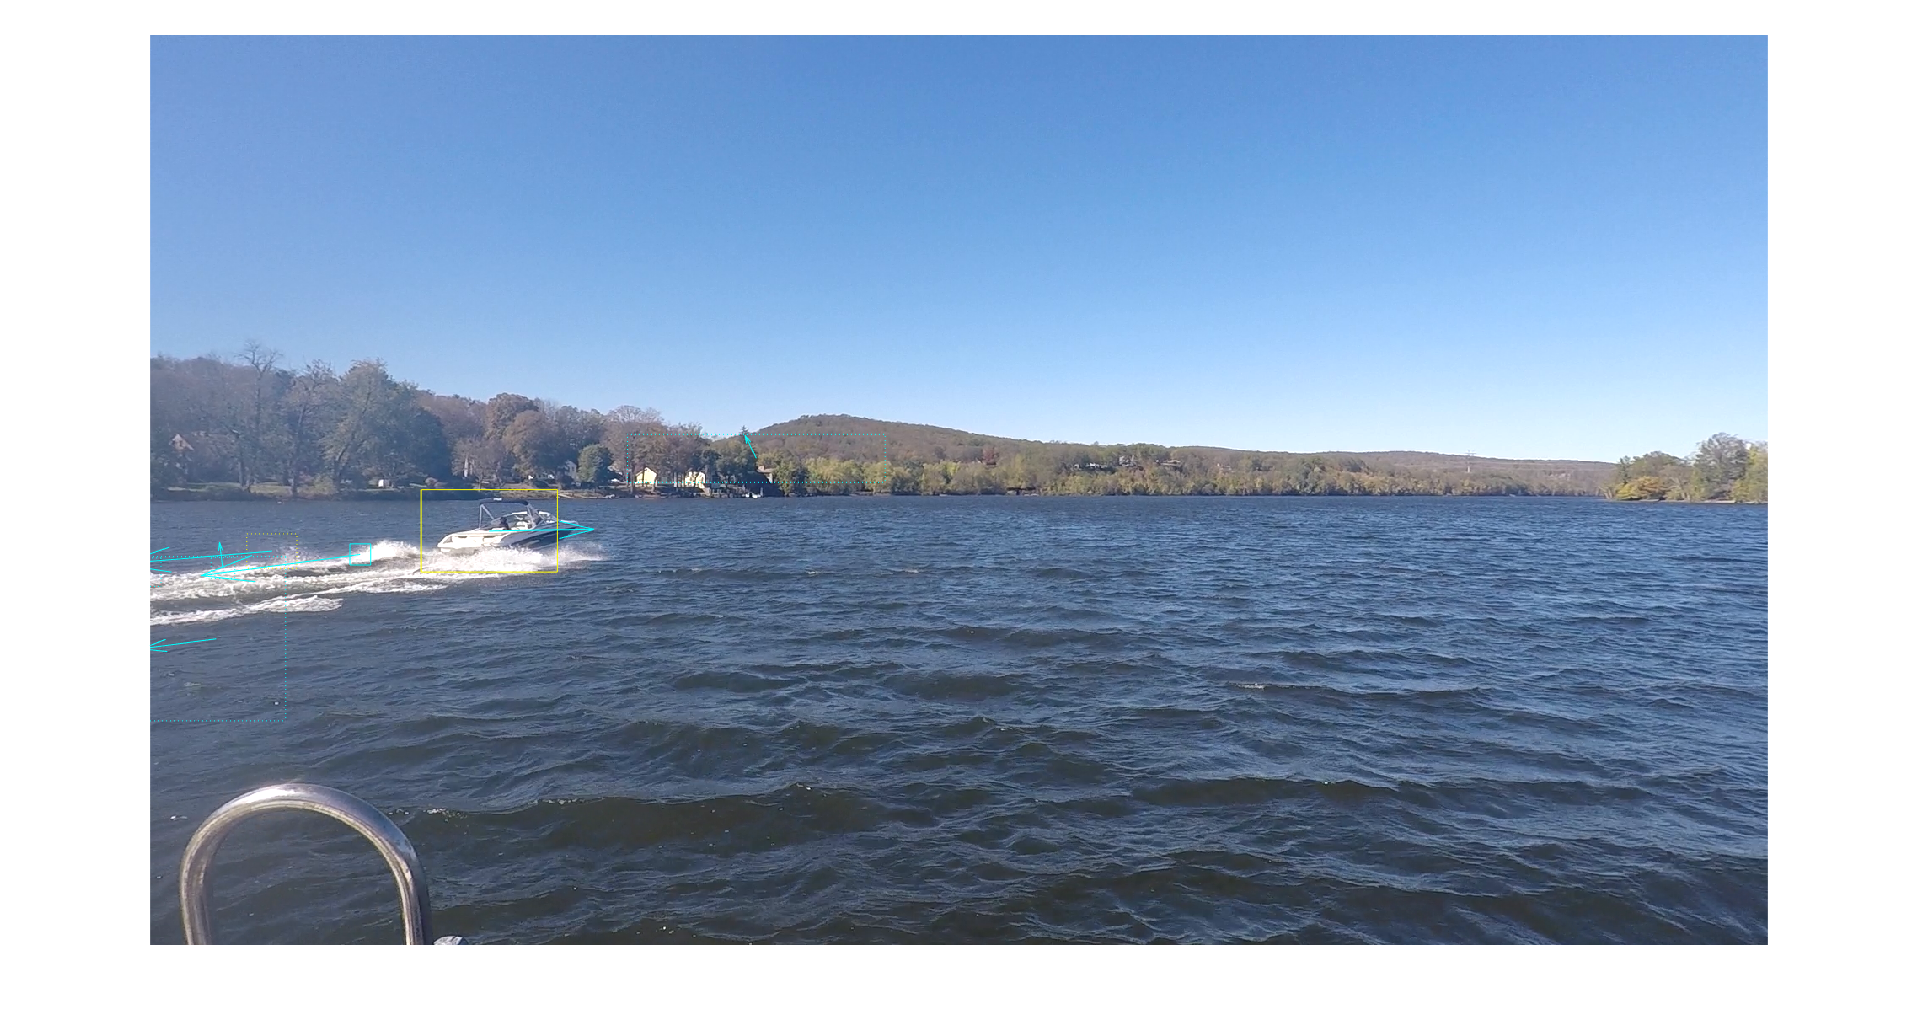
\includegraphics[width=\textwidth]{example_detection}
\caption{Sample frame of the whole stack running}
\label{fig:example_detection}
\end{figure}

In Figure \ref{fig:example_detection}, we see an individual frame from the
algorithm, where we have:
\begin{itemize}
\item The boat identified by a yellow (indicating that it has existed for at
      least 10 frames) solid (indicating high confidence) box with an arrow
      pointing leftwards, roughly in the direction of its movement.
\item Several solid and dashed boxes detecting the wake of the boat.
\end{itemize}

Longer videos can be found in our presentation:

\begin{description}
\item[\url{https://drive.google.com/file/d/1FoKWkp5xDSKwp5YyluKrclo_kGFU4gsg/view?usp=sharing}]
  In this video we have a longer view of the same boat as Figure
  \ref{fig:example_detection}
\item[\url{https://drive.google.com/file/d/1ndVSwF77_4va6U8rWT4FGJOXq1AjKL_Z/view?usp=sharing}]
  This has a slightly shorter capture of a different boat, indicating some
  degree of robustness to different individual instances
  \ref{fig:example_detection}
\end{description}

\subsection{Timing}

As we are interested in ultimately implementing some of these algorithms on our
actual robot, we are interested in the run time of our algorithms. These
are extremely rough numbers, from running only single-threaded on a laptop CPU,
but were reasonably consistent across runs:
\begin{itemize}
\item Around 3 seconds total per frame
\item Around 200 msec for the HSV segmentation
\item Around 1 second to call \texttt{opticalFlowFarneback} on the full
      1920x1080 image
\item Around half a second to perform the linear fit described in section
      \ref{expected_flow}
\item Around a second and a half spread out among other steps
\end{itemize}

The linear fit step in particular initially took up a substantial amount of
time, but we discovered that simply subsampling the data and only using around
10 percent of it worked almost as well while reducing the runtime to the half
second seen here.

The optical flow timing is exacerbated by the fact that we are running optical
flow on the entire, reasonably high-resolution, image. Were we to focus better
on interest regions, or simply use a lower resolution, we could likely achieve
substantially better results.

\subsection{Robustness}

\begin{figure}[H]
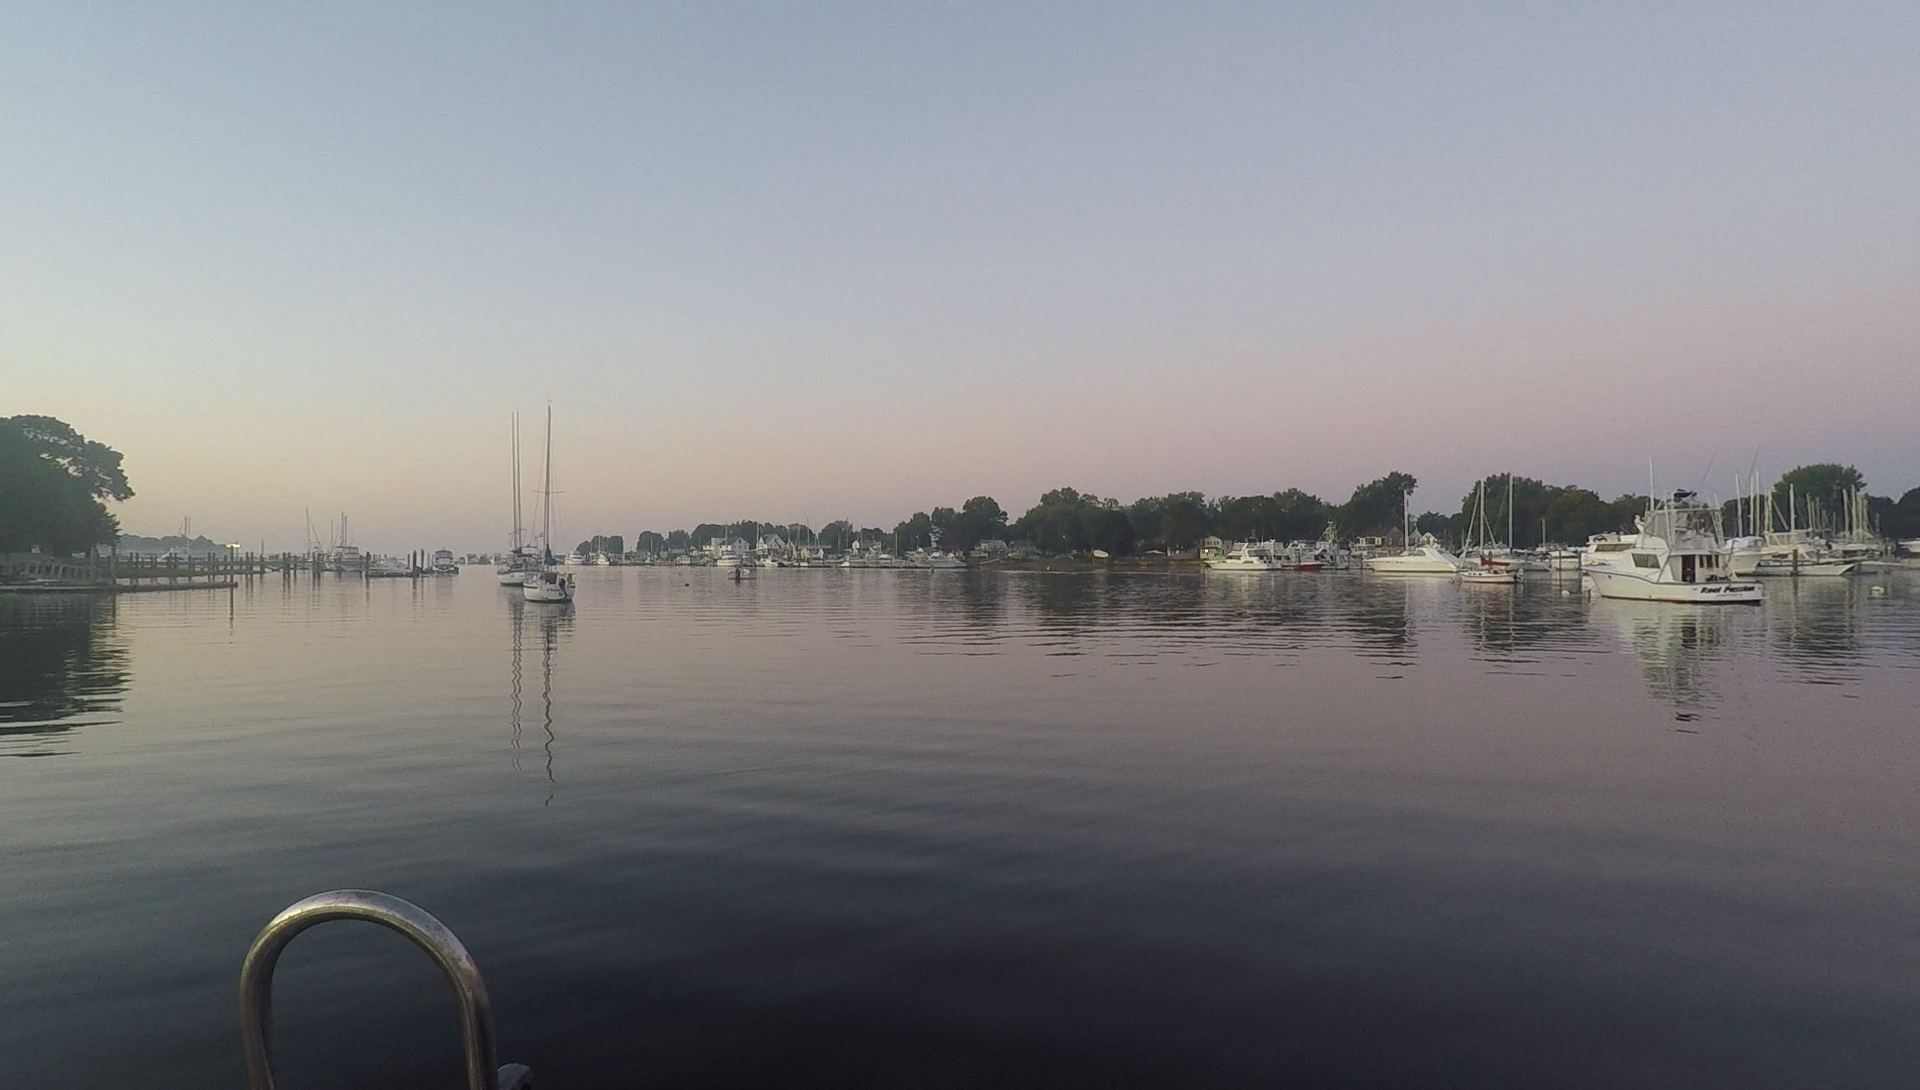
\includegraphics[width=12cm]{sample1}
\centering
\caption{Mirror-like water}
\label{fig:mirror}
\end{figure}

While the algorithms do work reasonably well for footage from these particular
conditions, we had troubles processing some parts of the data. In particular,
early mornings when not only was the sun interfering with the camera,
but also in situations such as Figure \ref{fig:mirror}, in which the water is
relatively flat (reducing texture) and highly reflective, meaning that it is no
longer particularly blue. The algorithm also struggles when pointed in the
 direction of the sun, as the reflections off of the water tend to oversaturate the image sensor.

\section{Future Work}

For future work, we need to actually improve the timing (as mentioned above) to
work in real time, improve robustness for a greater variety of conditions, and
to increase the generality to function on a less stable platform--our boat will
certainly be pitching and rolling substantially more than the platform we had
for this footage, and the weather conditions may be less ideal.

\bibliographystyle{ieeetr}
\bibliography{cite}

\end{document}
